\documentclass[11pt]{amsart}
\usepackage{geometry}                % See geometry.pdf to learn the layout options. There are lots.
\geometry{letterpaper}                   % ... or a4paper or a5paper or ... 
%\geometry{landscape}                % Activate for for rotated page geometry
%\usepackage[parfill]{parskip}    % Activate to begin paragraphs with an empty line rather than an indent
\usepackage{graphicx}
\usepackage{amssymb}
\usepackage{epstopdf}
\DeclareGraphicsRule{.tif}{png}{.png}{`convert #1 `dirname #1`/`basename #1 .tif`.png}



\begin{document}
\begin{figure}[htbp] %  figure placement: here, top, bottom, or page
   \begin{tabular}{c c}
   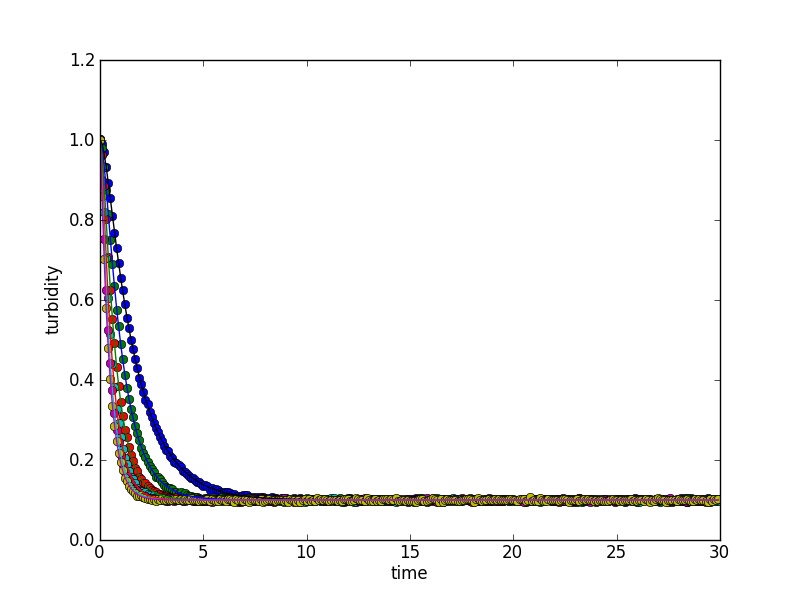
\includegraphics[width=3.5in]{turbidity6.png}& 
   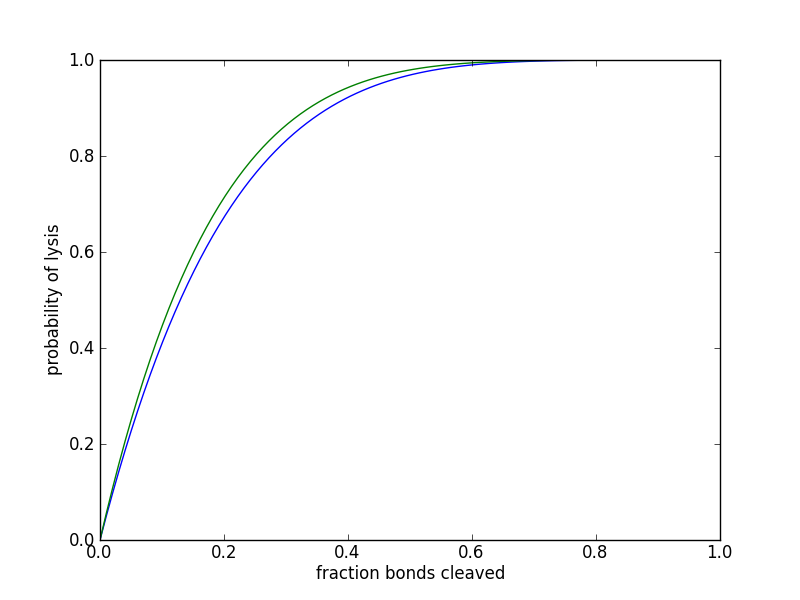
\includegraphics[width=3.5in]{susceptibility6.png}  
   \end{tabular}
\end{figure}

\begin{center}
    \begin{tabular}{ | c | c | c | c | c | c |}
    \hline
     & $k_{+}$ & $k_{-}$ & $k_{f}$ & $\alpha$ & $\beta$\\ \hline
    Actual & 0.5 & 2.1 & 0.5  & 1 & 5\\ \hline
    Estimated & 0.501 & 2.06 & 0.536  & 0.998 & 4.62 \\ \hline
    \hline
    \end{tabular}
\end{center}


\begin{figure}[htbp] %  figure placement: here, top, bottom, or page
   \begin{tabular}{c c}
   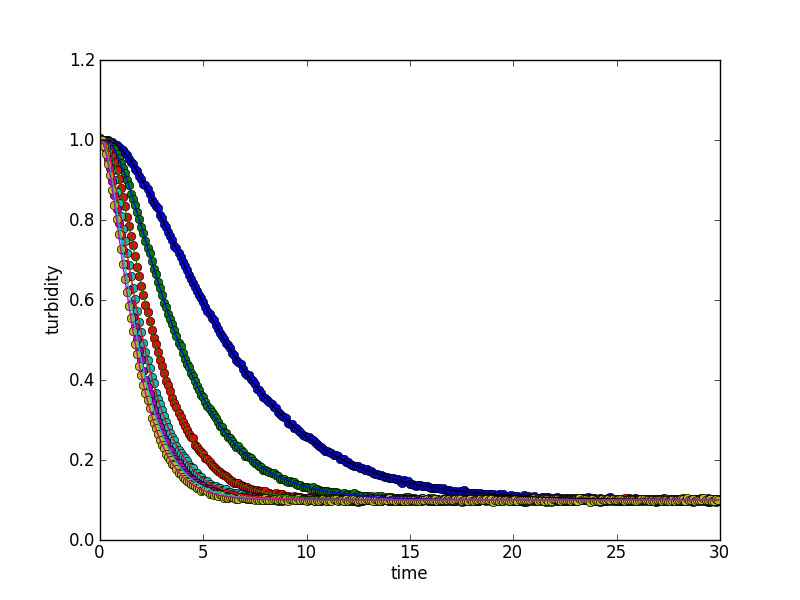
\includegraphics[width=3.5in]{turbidity2.png}& 
   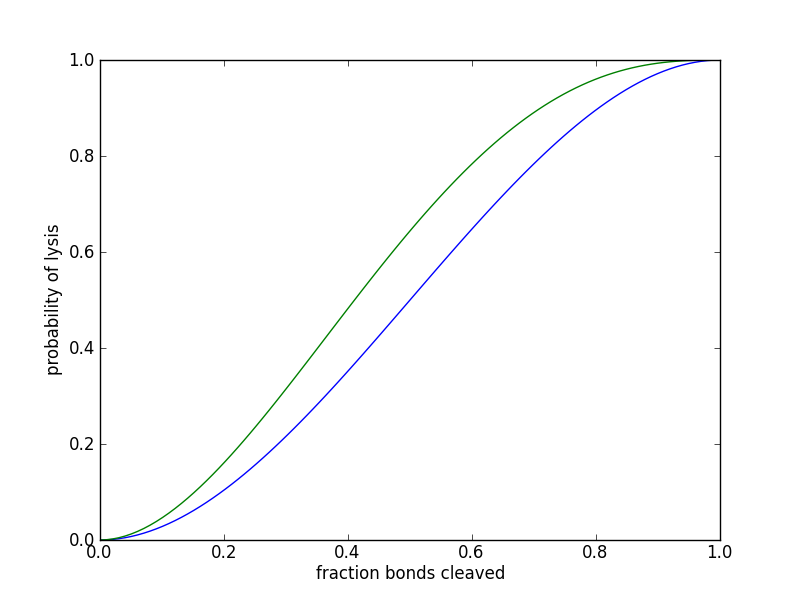
\includegraphics[width=3.5in]{susceptibility2.png}  
   \end{tabular}
\end{figure}

\begin{center}
    \begin{tabular}{ | c | c | c | c | c | c |}
    \hline
     & $k_{+}$ & $k_{-}$ & $k_{f}$ & $\alpha$ & $\beta$\\ \hline
    Actual & 1 &1.1 & 0.2  & 5 & 1\\ \hline
    Estimated & 2.01& 2.48  & 0.164  & 4.58 &1.33 \\ \hline
    \hline
    \end{tabular}
\end{center}

\begin{figure}[htbp] %  figure placement: here, top, bottom, or page
   \begin{tabular}{c c}
   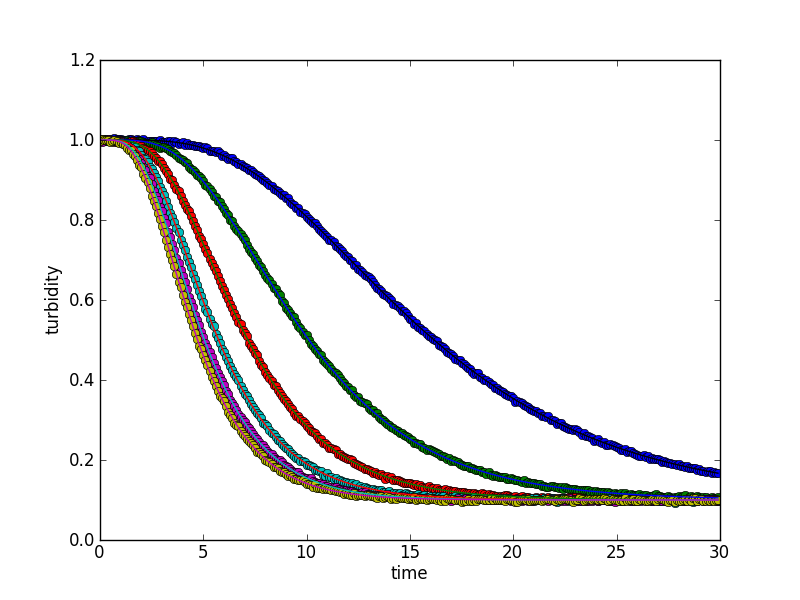
\includegraphics[width=3.5in]{turbidity4.png}& 
   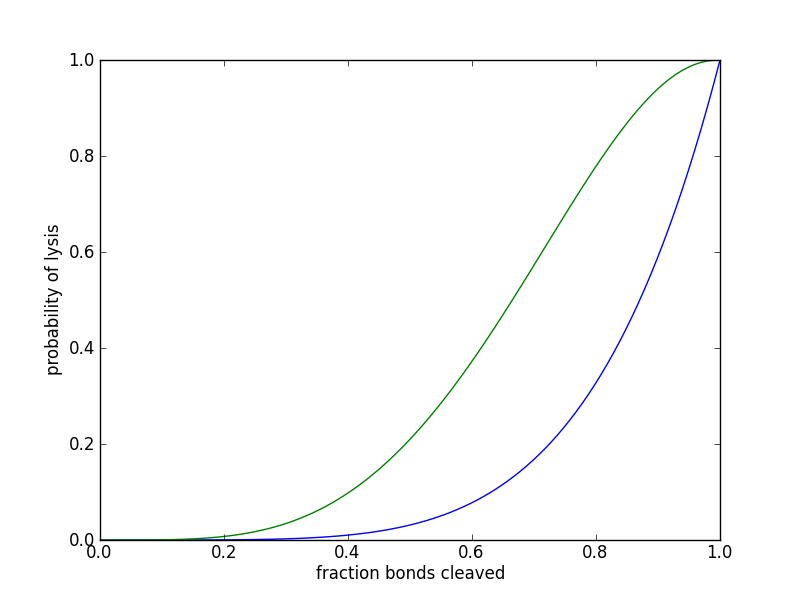
\includegraphics[width=3.5in]{susceptibility4.png}  
   \end{tabular}
\end{figure}

\begin{center}
    \begin{tabular}{ | c | c | c | c | c | c |}
    \hline
     & $k_{+}$ & $k_{-}$ & $k_{f}$ & $\alpha$ & $\beta$\\ \hline
    Actual & 0.5 & 2.1& 0.5  & 5 & 1\\ \hline
    Estimated & 0.958 & 4.57 & 0.261  & 0.998 & 4.62 \\ \hline
    \hline
    \end{tabular}
\end{center}





\end{document}  